\documentclass[12pt, a4paper]{report}
\usepackage{amsmath}
\usepackage{amssymb}
\usepackage{framed} % frame code if necessary
\usepackage{graphicx} % for importing images
\usepackage[margin=1in]{geometry} % set one inch margins
\usepackage{hyperref}

\author{Eric Leung}
\title{Final Research Project \\
	BMI 565/665 Python Scripting}
\date{December 8th, 2014}

\begin{document}

\maketitle

\section*{Part I: Identify Pathway Focus}

The first part of the project was completed with the \verb+odds.py+ file. We were also given three files to analyze.
\begin{itemize}
\item \verb+H5N1_VN1203_DE_Probes.txt+
\item \verb+H5N1_VN1203_UNIVERSE_Probes.txt+
\item \verb+KEGG_Pathway_Genes.txt+
\end{itemize}

Upon analysis, I found that there were six pathways that have a larger number of differentially expressed genes than would be expected by chance. This was determined with an odds ratio greater than 1.5.

\begin{table}[ht]
\begin{center}
\begin{tabular}{c|cc}
    ~                    & DE Genes & Non-DE Genes \\ \hline
    Target Pathway Genes & A        & B            \\
    Non-Pathway Genes    & C        & D            \\
\end{tabular}
\caption{A $2 \times 2$ contingency table of differential expression among target and non-target pathways used to calculate an odds ratio. \label{contingent}}
\end{center}
\end{table}

The odds ratio for each pathway was calculated with the following equation:
\begin{align}
OR = 
\frac{ \frac{A}{A+B} / \frac{B}{A+B} } 
{ \frac{C}{C+D} / \frac{D}{C+D}} =
\frac{A \times D}{B \times C}
\end{align}

The variables from the equation above reference those in Table~\ref{contingent}. A summary of the significant pathways are in Table~\ref{sigPaths} below. The variables ($A, B, C, D$) represent the number of genes based on each pathway that was being focused on. Thus, these variables will change depending on which pathway is focused on at the time.

\begin{table}[ht]
\begin{center}
\begin{tabular}{lc}
    Pathway                                         & Odds Ratio 	  \\ \hline
    ECM-receptor interaction                        & 2.2812   		  \\
    \textbf{RIG-I-like receptor signaling pathway}  & \textbf{2.2828} \\
    Focal adhesion                                  & 1.5999     	  \\
    Cytokine-cytokine receptor interaction          & 1.5165     	  \\
    Small cell lung cancer                          & 2.3641    	  \\
    Toll-like receptor signaling pathway            & 2.1792    	  \\
\end{tabular}
\caption{Significant pathways with odds ratios greater than 1.5 \label{sigPaths}}
\end{center}
\end{table}

The pathway I chose is ``RIG-I-like receptor pathway.'' It has an odds ratio of 2.2828, which is greater than 1.5, which we deem significant enough to study. An unhighlighted Figure~\ref{pathway} can be found at \url{http://www.kegg.jp/kegg-bin/show_pathway?hsa04622}.

\begin{figure}[ht]
\begin{center}
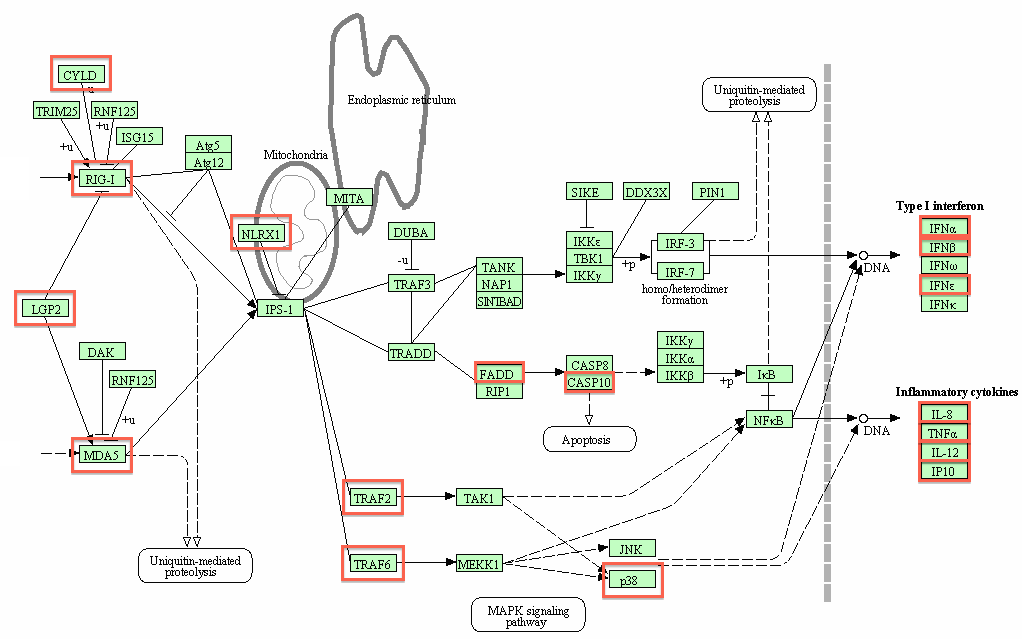
\includegraphics[width=16cm]{hsa04622.png}
\caption{RIG-I-like receptor signaling pathway for Homo sapiens with differentially expressed genes highlighted.}
\label{pathway}
\end{center}
\end{figure}

\section*{Part II: Examine Cross-Species Conservation of Pathway Genes}
% Discuss the relevance of the pathway to H5N1 infection. 
% Discuss why the conservation of the affected pathway might be important for the study of H5N1 (Hint: think about our use of model organisms to study infectious diseases). (20 points)

I studied the conservation of genes among Humans (\emph{Homo sapiens}), Mice (\emph{Mus musculus}), and Chimpanzees (\emph{Pan troglodytes}). Instead of taking genes from the ``KEGG Pathway Genes'' text file, I referenced the KEGG website \footnote{\url{http://www.kegg.jp/dbget-bin/www_bget?hsa04622}}. I relied on the KEGG API to search for and parse the right page to extract the list of genes.

I disregarded the file given because I found some ``genes'' listed for my pathway did not correspond to any human gene. Two were cDNA clones (AW511634 and AI423557), a partial CDS for a transcription factor (U88316), and another was from HeLa cells (U56433). Thus, I went straight to the source (KEGG) for the list of genes to study. Additionally, I came across a duplicate gene, but under difference names. Gene CR936771 in the KEGG pathways file is actually SIKE1, which is already in my list, but it is listed as SIKE, but SIKE1 is the official gene name, according to HGNC. 

\begin{figure}[ht]
\begin{center}
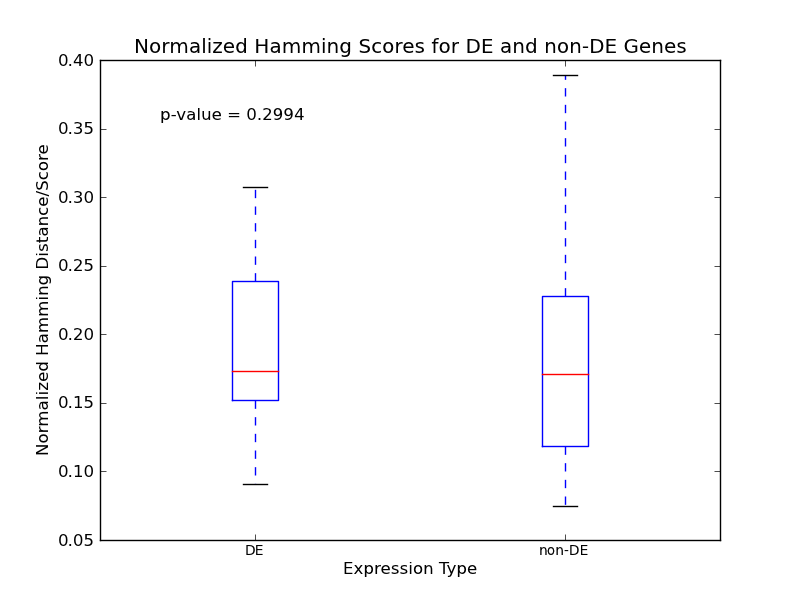
\includegraphics[width=12cm]{boxplot.png}
\caption{Boxplot of normalized Hamming distances for differentially expressed and non-differentially expressed genes in the RIG-I-like receptor pathway for Humans (\emph{Homo sapiens}), Mice (\emph{Mus musculus}), and Chimpanzees (\emph{Pan troglodytes}).\label{boxplot}}
\end{center}
\end{figure}

The decision to go to the KEGG database for the list of genes to study resulted in eighteen genes from the ``KEGG Pathway Genes'' file not being found for my pathway. As it was mentioned earlier, I found that I wouldn't have been able to find legitimate genes for five ``genes''. Thus, I did not search for thirteen genes. This may have had an effect on the final analysis. However, as you will see in the end, these thirteen missing genes must have had radical differences in them to change the overall statistical test.

I wanted to only compare genes that existed among all three species. This makes analysis easier instead of having to make a separate analysis for a pair of genes and all three genes. I found there was no significant difference between differentially expressed genes and non-differentially expressed genes in terms of Hamming distance among three different species (p-value $= 0.2994 > 0.05$).

One obstacle I found was how to search for the correct gene sequence to retrieve. If I used the Entrez E-Utils and searched by gene name, I could only get close to the correct gene I wanted (a RefSeq mRNA sequence), but it would vary from each gene. I was not satisfied with retrieving any sequence (e.g. predicted or anything not RefSeq if possible). So I tried to find other, more precise ways of searching. This is another reason why I decided to reference the KEGG database because before each gene in a specified pathway is an ID that can be search precisely in Entrez to get the RefSeq database. 

\section*{H5N1 Infection Reflection}
% Discuss why the conservation of the affected pathway might be important for the study of H5N1 (Hint: think about our use of model organisms to study infectious diseases). (20 points)

% Specific families of pattern recognition receptors are responsible for detecting viral pathogens and generating innate immune responses. Non-self RNA appearing in a cell as a result of intracellular viral replication is recognized by a family of cytosolic RNA helicases termed RIG-I-like receptors (RLRs). The RLR proteins include RIG-I, MDA5, and LGP2 and are expressed in both immune and nonimmune cells. Upon recognition of viral nucleic acids, RLRs recruit specific intracellular adaptor proteins to initiate signaling pathways that lead to the synthesis of type I interferon and other inflammatory cytokines, which are important for eliminating viruses.

The H5N1 infection is a type of bird flu. The pathway I chose (RIG-I-like receptor pathway) is ``responsible for detecting viral pathogens and generating innate immune responses''\footnote{\url{http://www.kegg.jp/dbget-bin/www_bget?hsa04622}}. This can be very important in responding to the onset of the flu virus, which supports the reason why this pathway's genes are differentially expressed.

Conservation of the affected pathway in model organisms is important when studying H5N1 because successful treatments on affected model organisms will have more confidence in translating the successful treatments to humans compared to distantly related model organisms.

\end{document}